% !TEX root = thesis.tex
%
% ------------------------------------  --> cover title page

\pdfbookmark[0]{Cover}{Cover}
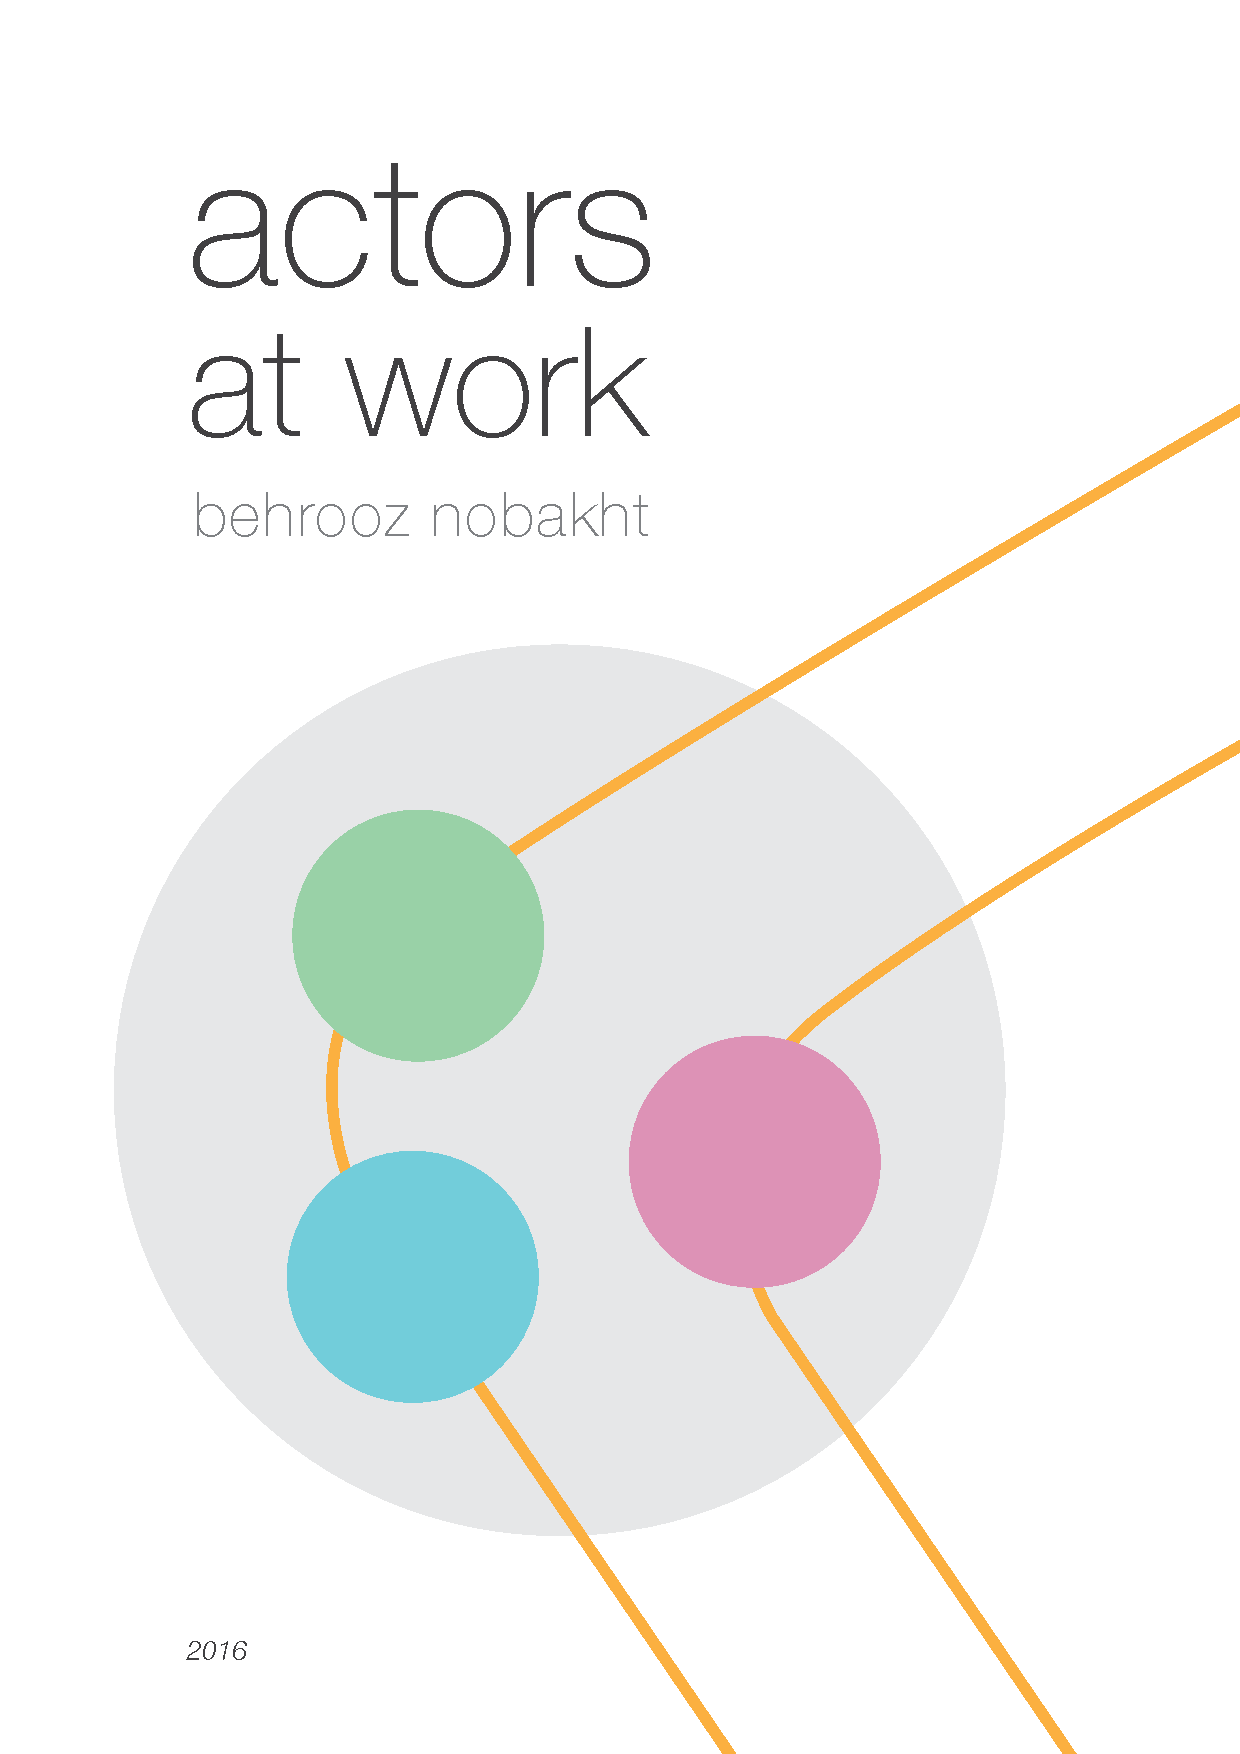
\includepdf{cover.pdf}

% \begin{titlepage}
% 	\pdfbookmark[0]{Cover}{Cover}
% 	\flushright
% 	\hfill
% 	\vfill
% 	{\LARGE\thesisTitle \par}
% 	\rule[5pt]{\textwidth}{.4pt} \par
% 	{\Large\thesisName}
% 	\vfill
% \end{titlepage}

% ------------------------------------  --> main title page
\begin{titlepage}
	\pdfbookmark[0]{Official Title}{Official Title}
	\tgherosfont
	\centering

	{\Large \thesisUniversity} \\[4mm]
	
\includegraphics[width=6cm]{figs/ullogo} \\[2mm]
	\textsf{\thesisUniversityDepartment} \\
	\textsf{\thesisUniversityInstitute} \\
	\textsf{\thesisUniversityGroup} \\

	\vfill
	{\large \thesisSubject} \\[5mm]
	{\LARGE \color{ctcolortitle}\textbf{\thesisTitle} \\[10mm]}
	{\Large \thesisName} \\

	% \vfill
	% \begin{minipage}[t]{.27\textwidth}
	% 	\raggedleft
	% 	\textit{1. Reviewer}
	% \end{minipage}
	% \hspace*{15pt}
	% \begin{minipage}[t]{.65\textwidth}
	% 	{\Large \thesisFirstReviewer} \\
	%   	{\small \thesisFirstReviewerDepartment} \\[-1mm]
	% 	{\small \thesisFirstReviewerUniversity}
	% \end{minipage} \\[5mm]
	% \begin{minipage}[t]{.27\textwidth}
	% 	\raggedleft
	% 	\textit{2. Reviewer}
	% \end{minipage}
	% \hspace*{15pt}
	% \begin{minipage}[t]{.65\textwidth}
	% 	{\Large \thesisSecondReviewer} \\
	%   	{\small \thesisSecondReviewerDepartment} \\[-1mm]
	% 	{\small \thesisSecondReviewerUniversity}
	% \end{minipage} \\[5mm]
	% \begin{minipage}[t]{.27\textwidth}
	% 	\raggedleft
	% 	\textit{3. Reviewer}
	% \end{minipage}
	% \hspace*{15pt}
	% \begin{minipage}[t]{.65\textwidth}
	% 	{\Large \thesisThirdReviewer} \\
	%   	{\small \thesisThirdReviewerDepartment} \\[-1mm]
	% 	{\small \thesisThirdReviewerUniversity}
	% \end{minipage} \\[10mm]
	% \begin{minipage}[t]{.27\textwidth}
	% 	\raggedleft
	% 	\textit{Supervisors}
	% \end{minipage}
	% \hspace*{15pt}
	% \begin{minipage}[t]{.65\textwidth}
	% 	\thesisFirstSupervisor\ and \thesisSecondSupervisor
	% \end{minipage} \\[10mm]

% --- From Leiden University Template

\begin{center}
% \printtitle
\par\vspace {2.1cm}
{\large \textsc Proefschrift}
\par\vspace {1.5cm}
{\large ter verkrijging van\\[.5cm]
de graad van doctor aan de Universiteit Leiden\\[.5cm]
\makebox[0pt][c]{op gezag van de Rector Magnificus prof. dr. C. J. J. M. Stolker,}\\[.5cm]
volgens besluit van het College voor Promoties\\[.5cm]
te verdedigen %in de Aula der Universiteit \\        
op woensdag 18 december 2013\\[.5cm]
klokke 10.00 uur \\[.5cm] }
\par\vspace {1cm} {\large door}
\par \vspace {.5cm} % Note: next should be your _full_ name
{\Large Behrooz Nobakht}    
\par%\vspace {1cm} % and your birthplace
{\large geboren te Tehran, Iran, in 1981} %PERSONALIZE
% Note: include your country of birth IF AND ONLY IF you were not born
% in the Netherlands
\end{center}
%%the fourth page: promotores, ISBN etc.
\clearpage
\noindent%
{\Large\textbf{PhD Committee}}\\[.5cm]

\begin{tabular}{lll}
Promotor:    & Prof.\ Dr.\ F.S. de Boer & \\
Co-promotor: & Dr.\ C. P. T. de Gouw & \\[12pt]
Other members:\\
& Prof.\ Dr.\ F. Arbab & \\
& Dr.\ M.M. Bonsangue & \\
& Prof.\ Dr.\ E. B. Johnsen & University of Oslo, Norway\\
& Prof.\ Dr.\ M. Sirjani & Reykjavik University, Iceland\\
& Dr.\ P.Y.H. Wong & Travelex, United Kingdom\\
\end{tabular}

\vfill
\vspace{5.5cm}

\hspace{-0.5cm}
\begin{tabular}{lll}

\includegraphics[height=0.8cm]{figs/cwi.png} &

\includegraphics[height=1.2cm]{figs/envisage-logo} &
\end{tabular}
% \\ \\

% If you're supported by NWO adapt the following 6 lines;
% otherwise simply delete them.
%
\noindent
The work reported in this thesis has been carried out at the Center for Mathematics and Computer Science (CWI) in Amsterdam and Leiden Institute of Advanced Computer Science at Leiden University.
This research was supported by the European FP7-231620 project ENVISAGE on Engineering Virtualized Resources.
\par\vspace {1cm}

% If you want to add CIP data (a summary of all the data used in
% library catalogs in a standard format), uncomment the following
% three lines and add the CIP data in between
%
%\noindent%
%{\tt CIP gegevens}                                 % PERSONALIZE
%\\[4ex]                                            %PERSONALIZE

%Copyright and accreditation stuff, plus ISBN
%
\noindent%
% Copyright: put your name here
Copyright \copyright\ 2016 by Behrooz Nobakht. All rights reserved. \\ [2ex] %PERSONALIZE
% Cover design, if your cover was designed by someone else
%The cover illustration depicts a real-time solution to the dining philosophers problem.
%This solution is referred to as ``A Late Philosopher'' in Section \ref{sec::late}.
% \\
%Cover design by Samira Sedghi.\\                       %PERSONALIZE
%Maybe some additional info on the production of the dissertation.
%Don't forget your printing shop
%Printed and bound by your printer.\\[2ex]           %PERSONALIZE
%ISBN number: ask your faculty library how to obtain one
%ISBN:  978-90-6464-445-0                              %PERSONALIZE

% Dedication, table of contents and acknowledgements
% are handled in the main file


	\thesisDate \\

\end{titlepage}


% ------------------------------------  --> lower title back for single page layout
\hfill
\vfill
{
	\small
	\textbf{\thesisName} \\
	\textit{\thesisTitle} \\
	\thesisSubject, \thesisDate \\
	Promoter: Prof. Dr. \thesisFirstReviewer \\
	% Supervisor(s): \thesisFirstSupervisor \\[1.5em]
	Cover Design: Ehsan Khakbaz \jtt{<ehsan@khakbaz.com>} \\[1.5em]
	Built on \jtt{\gitAuthorIsoDate} from \jtt{\gitHash} at \\
	\url{https://github.com/nobeh/thesis} \\[1.5em]
	\textbf{\thesisUniversity} \\
	\textit{\thesisUniversityGroup} \\
	\thesisUniversityInstitute \\
	\thesisUniversityDepartment \\
	\thesisUniversityStreetAddress \\
	\thesisUniversityPostalCode\ and \thesisUniversityCity
}
